
Este capítulo apresenta, inicialmente, os detalhes do módulo de escalonamento do BioNimbuZ. Posteriormente, discorre sobre a implementação, mostrando alguns dos problemas encontrados durante o desenvolvimento e como eles foram solucionados. A terceira seção aborda a adição de tarefas que utilizam a \acrshort{GPU} no BioNimbuZ, e na última parte deste capítulo são descritos os testes que podem ser feitos e o resultados obtidos a partir do novo escalonador.

\section{Sistema de Escalonamento do BioNimbuZ}

O Serviço de Escalonamento é implementado no BioNimbuZ como um serviço da Camada de Núcleo (veja a Figura \ref{Arquitetura}), de acordo com o subsistema mostrado na Figura \ref{SubsistemaDeEscalonamento}. A interface \textit{services} define métodos para a inicialização, o término de serviços e os métodos para comunicação com o \textit{Zookeeper} \cite{Zookeeper}. 
\begin{figure}[htbp]
	%	\centerline{\includegraphics[scale=0.04]{img/EscalonadorProposto.png}}
	\centerline{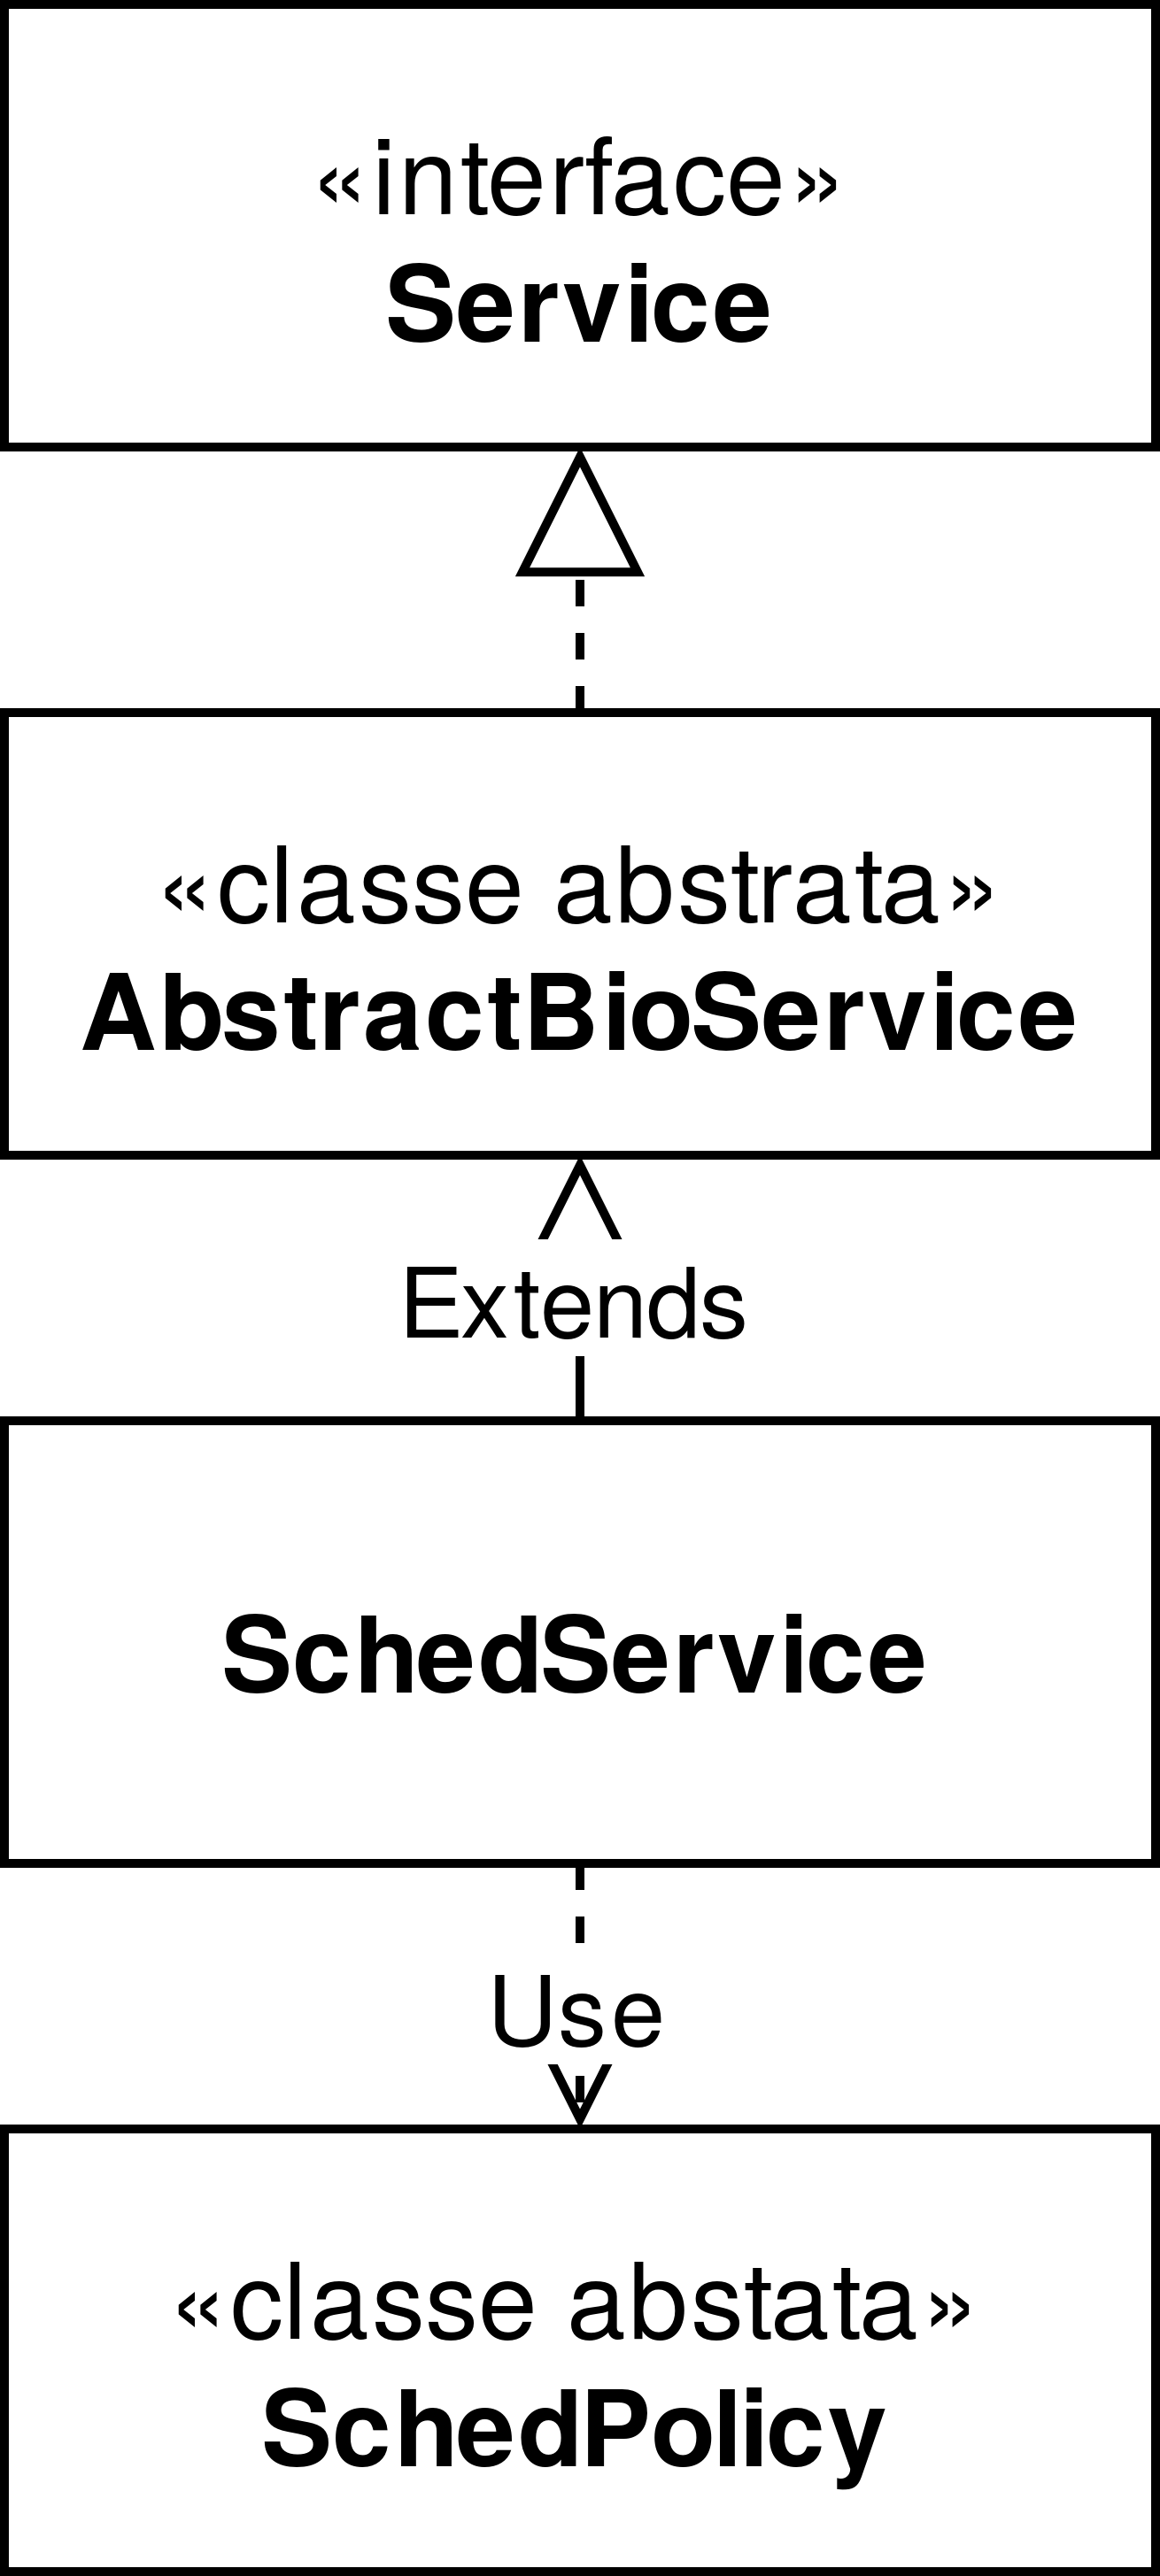
\includegraphics[width=2.8cm]{img/SubsistemaDeEscalonamento.png}}
	\caption{Subsistema de Escalonamento do BioNimbuZ.}
	\label{SubsistemaDeEscalonamento}
\end{figure}
A classe \textit{AbstractBioService} define funcionalidades comuns aos serviços do BioNimbuZ, em especial, a comunicação entre as máquinas que compõem a plataforma e o padrão de projeto \textit{observer}, utilizado para notificação de eventos.

A classe \textit{SchedService} é a responsável por prover o serviço de escalonamento em si, entretanto, para permitir a existência de várias políticas de escalonamento, internamente ela utiliza instâncias da classe abstrata \textit{SchedPolicy}, que implementam cada uma das distintas políticas de escalonamento existentes, conforme mostrado na Figura \ref{ArquiteturaAtual}.

Essas políticas de escalonamento são implementadas por meio da definição dos seguintes métodos herdados de \textit{SchedPolicy}:
\begin{itemize}
%	\item \textit{schedule}, que recebe como arguento uma lista de \textit{Jobs} para ser escalonado e retorna um mapeamento de \textit{Job} para um conjunto de máquinas as quais realizarão a computação.
	\item \textit{schedule}, que realiza o escalonamento inicial propriamente dito;
	\item \textit{relocate}, o qual realoca um processamento que está em execução;
	\item \textit{cancelJobEvent}, cujo objetivo é reportar ao escalonador o cancelamento de um \textit{job};
	\item \textit{jobDone}, que informa ao escalonador que um \textit{job} terminou.
\end{itemize}

\begin{figure}[htbp]
	\centerline{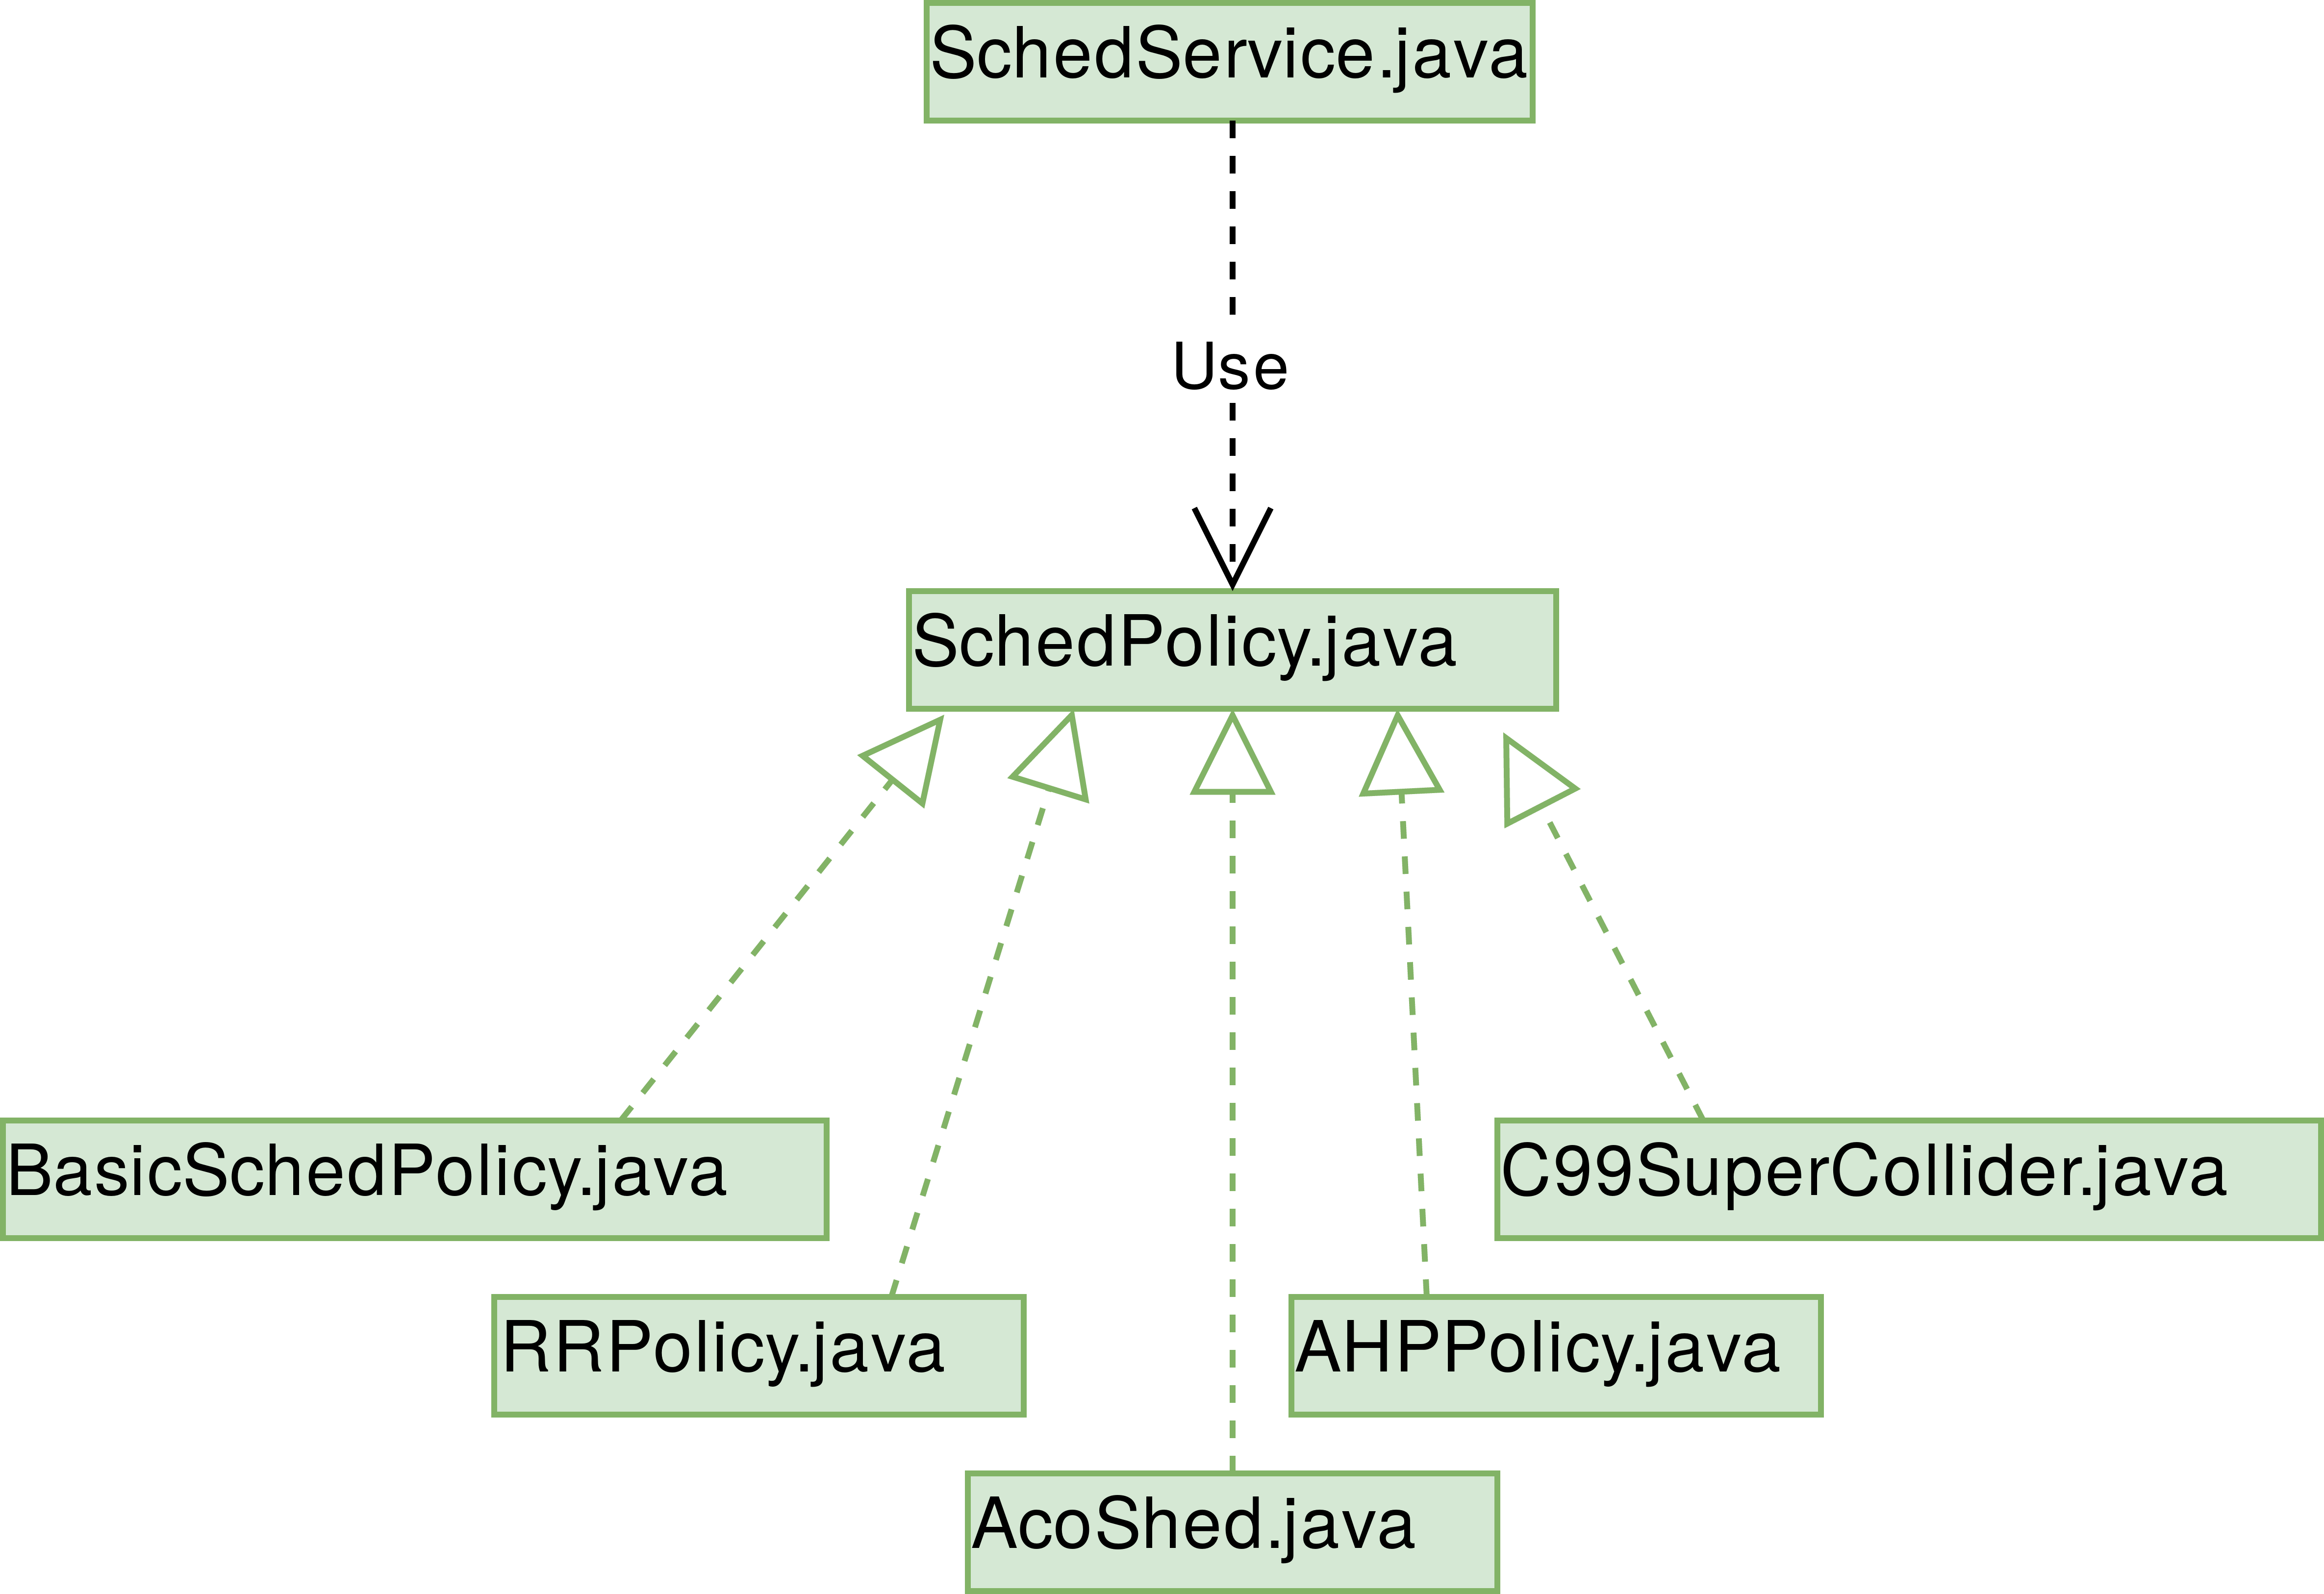
\includegraphics[width=12cm]{img/ArquiteturaAntesHoriz.png}}
	\caption{Subsistema de Escalonamento do BioNimbuZ.}
	\label{ArquiteturaAtual}
\end{figure}


\section{Implementação do Escalonador Proposto}

Por motivos de familiaridade com a linguagem de programação, o escalonador proposto foi implementado em C++. Para ter compatibilidade com os demais componentes do software, classes auxiliares, como a que representa os \textit{Jobs} e as \acrshort{VM}s instanciáveis tiveram equivalentes escritos em C++. Além disso, dois outros problemas surgiram, que foram como iniciar o escalonador C++, e como ele deve se comunicar com os demais componentes da plataforma. O primeiro problema foi resolvido por meio de pesquisa na \acrfull{API} do Java, utilizando as classes \textit{Process}\cite{JavaProcess}, \textit{Runtime}\cite{JavaRuntime} e \textit{ProcessBuilder}\cite{JavaProcessBuilder}, os quais permitem executar comandos de terminal, o que possibilitou a execução da parte C++ do escalonador.

O problema da comunicação do C++ com o Java é mais difícil, pois há várias formas de fazer. Por exemplo, o uso de classes \textit{wrappers} que usam \textit{handles}, que são objetos cujo objetivo é manipular estruturas que não são nativas da linguagem\cite{CppJavaHandle}. Uma outra forma documentada é através do uso do \acrfull{JNI}, que é uma outra forma existente no qual, através do uso de \textit{handles}, é chamado o código C++ num programa Java\cite{CppJavaJNI}. Além disso, existem variações deste método utilizando bibliotecas que buscam simplificar o gerenciamento do \textit{handle}. Como as formas pesquisadas para fazer tal comunicação aparentam não chegar a um consenso, decidiu-se então utilizar formas mais genéricas de comunicação entre processos, o qual surgiu a ideia de usar \textit{sockets} para fazer a comunicação.

\textit{Socket} é uma abstração que sistemas operacionais fazem para permitir que programas tenham acesso à rede. \iffalse Os sistemas operacionais organizam os \textit{sockets} disponíveis e portas, essa organização de portas também é utilizada por protocolos de rede, \fi O sistema de portas permite diferenciar em um computador qual dos programas interessados está enviando ou deve receber a mensagem. %E um truque que pode ser feito usando a pilha de rede \acrshort{TCP/IP} é enviar mensagens para o próprio computador, através da interface de rede de \textit{loopback}. E esse é um método efetivo de comunicação entre processos distintos.

\begin{figure}[htbp]
	\centerline{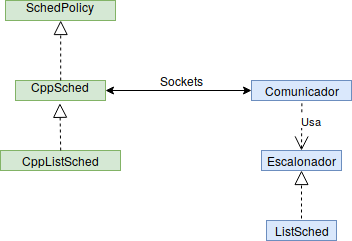
\includegraphics[scale=0.7]{img/Proposta.png}}
	\caption{Arquitetura de Classes do Escalonador Implementado.}
	\label{ArquiteturaProposta}
\end{figure}

Uma vez decidido o uso de \textit{sockets}, faltava decidir qual seria o protocolo da camada de rede e de transporte. Na camada de rede o principal protocolo existente é o \acrfull{IP}, entretanto, existem duas versões: o IPv4\cite{ipv4rfc} e o IPv6\cite{ipv6rfc}, sendo que o último é mais recente e permite um maior número de dispositivos na rede, por isso essa foi a versão utilizada na implementação. Quanto à camada de transporte, os candidatos eram o \acrshort{TCP}\cite{tcp_rfc} e o \acrshort{UDP}\cite{udp_rfc}. O \acrshort{TCP} provê uma série de garantias ao usuário dos pacotes que serão transmitidos pela rede ao custo de \textit{overhead}, mas como apenas será utilizado para comunicação em \textit{loopback}. O \acrshort{UDP} é mais simples e enxuto, sendo o escolhido como protocolo da camada de transporte neste trabalho.

%Uma dificuldade encontrada durante a implementação do uso de \textit{sockets}, foi como utilizar o IPv6, pois, especialmente para a linguem C, há pouca documentação disponível sobre, por mais que exista boa documentação sobre o uso de \textit{sockets} IPv4.


Como pode ser observado na Figura \ref{ArquiteturaProposta}, para a implementação desse sistema de comunicação no BioNimbuZ, desenvolveu-se a classe abstrata \textit{CppSched} que herda de \textit{SchedPolicy}, responsável por fazer a inicialização do programa C++ e pelo \textit{handshake} entre os processos C++ e Java, permitindo que futuros escalonadores em C++ não precisem repetir este processo. Da classe \textit{CppSched} herda o método \textit{GetSchedPolicy}, utilizado para informar qual escalonador C++ deve ser utilizado.

\begin{figure}[htbp]
	\centerline{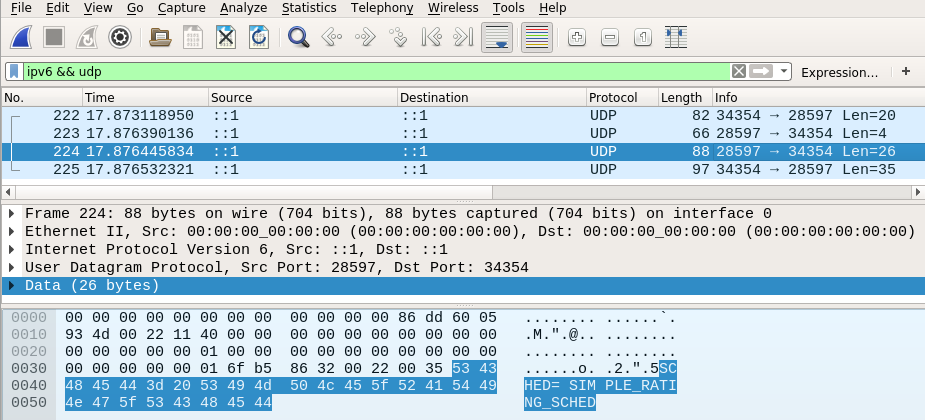
\includegraphics[width=13cm]{img/Handshake3.png}}
	\caption{Handshake entre a parte Java e C++ do Escalonador.}
	\label{Handshake}
\end{figure}

O programa C++ é composto pela classe Comunicador, que inicializa seu \textit{socket} e inicia a conversa com o processo Java, cuja porta de comunicação é recebida pela linha de comando. Durante o \textit{handshake} é definido qual filho da classe virtual Escalonador será usado. Em prol da simplicidade e da performance, buscou-se minimizar a comunicação entre os processos C++ e Java. Assim, após a inicialização, o processo C++ se comporta similarmente à um servidor \acrshort{DNS}\cite{dns_rfc}, ficando em espera por solicitações de escalonamento, e responde às requisições sem manter estado internamente.

\section{Aplicação Testada no BioNimbuZ}

%No início do projeto, imaginava-se que os \textit{workflows} existentes no BioNimbuZ seriam capazes de tirar proveito da \acrshort{GPU}, pressuposto que se revelou falso ao longo do desenvolvimento do projeto. Logo fez-se necessário procurar por programas de uso geral que utilizem a \acrshort{GPU}, uma atividade que se revelou simples. 
Para os testes foi escolhido o programa XMR-Stak\cite{xmr_stak}, um programa de mineração de criptomoedas, que são artefatos digitais desenvolvidos como meio de troca, que utilizam criptografia para prover segurança e integridade à transações\cite{crypto_currencies}. Esse software de mineração, em específico, foi escolhido pelo fato de ser software livre e, por isso, ter seu código fonte disponível publicamente, além de ser multiplataforma e capaz de executar tanto em \acrshort{CPU} quanto em acrshort{GPU}.

A mineração de criptomoedas é a atividade de buscar \textit{nouces}, isto é, uma sequência aleatória de bytes, que quando inserido junto de um possível futuro bloco de uma \textit{blockchain}, que é uma lista distribuída para armazenamento de registros, numa função de \textit{hash} criptográfico, gera um \textit{hash} que atenda a algum critério de dificuldade, geralmente um valor específico no início. Quando é encontrado um \textit{digest}, uma saída da função de \textit{hash}, que atende ao critério, tal bloco é adicionado na \textit{blockchain}, e o responsável pela máquina que encontrou a resposta é recompensado em criptomoeda.

Assim, uma vez testado a plataforma na \acrshort{VM}, é hora de testar em equipamento real, pois as máquinas virtuais não possuem acesso à \acrshort{GPU}, a não se quando utilizado \textit{\acrshort{GPU} Passthrough}, que é uma técnica que permite redirecionar o controle de uma \acrshort{GPU} física para uma máquina virtual. Uma das maiores barreiras para o \textit{\acrshort{GPU} Passthrough} é que ele requer pelo menos duas placas de vídeos, pois tanto o sistema hóspede quanto o sistema hospedeiro devem ter cada um sua \acrshort{GPU}.

%\subsection{Da \acrshort{VM} para a máquina de testes}

Após a plataforma apresentar correto funcionamento, toda a instalação seria clonada num \textit{flash drive} \acrshort{USB} capaz de inicializar, para tal o \textit{bootloader}, \textit{software} responsável por determinar como o sistema será inicializado, ser reparado para que seja capaz de inicializar a partir do dispositivo móvel de armazenamento. O sistema precisa ser clonado pois usa pacotes de versões diferentes do sistema operacional Debian\cite{Debian}, porque o XMR-Stak utiliza a biblioteca de processamento paralelo \acrshort{CUDA}\cite{CUDA}, da Nvidia\cite{NVIDIA},e essa biblioteca requer o uso da versão 6 do compilador \acrshort{GCC}\cite{GCC}, disponível no repositório da versão \textit{stable} do Debian. A biblioteca do CUDA está disponível na versão \textit{unstable} do sistema operacional. O \acrshort{CUDA} foi retirado da versão \textit{testing} do Debian por causa dessa dependência da versão 6 do \acrshort{GCC}, que é considerada desatualizada\cite{CUDA_BUGREP}.


\section{Implantação no BioNimbuZ}

O escalonador foi, inicialmente, desenvolvido utilizando apenas o subsistema de escalonamento do BioNimbuZ, para que testes fossem feitos com rapidez. Após testes que comprovaram o funcionamento do escalonador, como o da Figura \ref{Handshake}, utilizou-se uma máquina virtual para fazer a implantação do escalonador desenvolvido de volta ao BioNimbuZ, pois a instalação do BioNimbuZ requer instalação de programas que podem, mesmo que seja incomum, conflitar ou apresentar erros em iterações com o resto do sistema operacional. Um exemplo que ocorreu durante o desenvolvimento foi uma atualização do sistema operacional, Debian\cite{Debian} Testing\cite{DebianTesting}, que causou erros em tempo de execução no \acrfull{IDE} Eclipse\cite{JavaEclipse}, relativos à interface gráfica. O mecanismo de \textit{snapshots} providos pelo software de gerenciamento de \acrshort{VM}s Virtualbox\cite{VirtualBox} se revelou realmente útil nessa circunstância, como pode ser visto na Figura \ref{Snapshots}.

\begin{figure}[htbp]
	\centerline{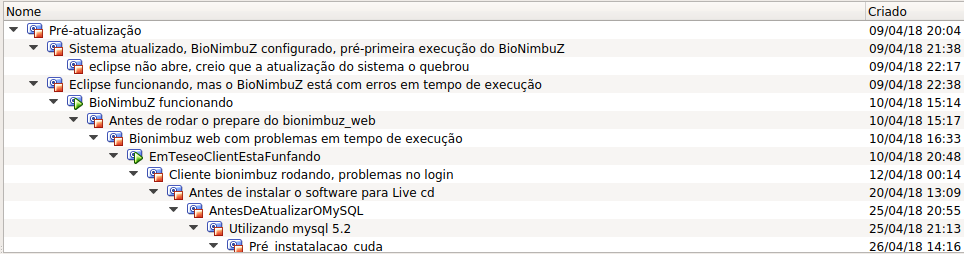
\includegraphics[width=12cm]{img/Snapshots.png}}
	\caption{Parte dos \textit{Snapshots} existentes na \acrshort{VM} de Implantação.}
	\label{Snapshots}
\end{figure}

Nos primeiros testes de funcionamento do BioNimbuZ, percebeu-se um erro no qual era possível cadastrar novo usuários, mas não era possível logar na plataforma, apenas aparecendo a mensagem "Erro Interno". Pesquisa nos arquivos de \textit{log} mostraram que o BioNimbuZ não estava conseguido criar a maioria de suas tabelas no \acrfull{SGBD} MySQL, devido ao tamanho de limite de linha das tabelas, causado pele junção de vários campos para armazenamento de \textit{strings} e o fato do \acrshort{SGBD} utilizar 4 bytes para codificar cada caractere. Após pesquisar possíveis soluções, incluindo atualização do MySQL, decidiu-se criar manualmente as tabelas que apresentavam esse problema, reduzindo o tamanho de alguns campos de texto, solução que resolveu o problema sem perda aparente de funcionalidade.

Outro problema enfrentado durante o desenvolvimento foi que \textit{workflows} não eram enviados para execução quando solicitado, os \textit{logs} apenas informavam "Error: NULL", sem maiores informações para solucionar o problema, que foi identificado como uma inicialização incompleta do BioNimbuZ por causa que a \textit{thread} que inicializava a plataforma ficava à espera de uma mensagem que já havia sido recebida no \textit{socket}, porém incorretamente descartado porque no Java, para se comparar a mensagem recebida com o que se espera, é necessário explicitar a codificação tanto da mensagem recebida quando do texto esperado.

Mais uma adversidade ocorrida durante a implantação é que quando se seleciona o computador local para executar uma tarefa, esse computador não é listado entre as máquinas disponíveis para o escalonamento. Assim, nenhuma outra máquina for escolhida para escalonamento, a requisição que o escalonador recebe não disponibiliza máquinas para escalonar, fazendo com que o escalonamento falhe.

\section{Métricas para Testes}

Uma vez preparado o dispositivo portátil de testes, o passo seguinte seria realizar uma série de testes com o objetivo de coletar o máximo de dados possíveis na versão desenvolvida do BioNimbuZ. O sistema de \textit{log} do BioNimbuZ já nos fornece informação sobre a duração da execução dos \textit{jobs} de um \textit{workflows}, além do tempo gasto no subsistema de escalonamento. O código de instrumentação pode ser inserido na parte C++ do escalonador para calcular o tempo gasto apenas no escalonamento, excluindo tempo gasto na serialização e na desserialização das mensagens entre as partes C++ e Java da plataforma. Dessa forma, se um \textit{software} de captura de pacotes for utilizado, por exemplo o Wireshark\cite{Wireshark}, é possível verificar o total de tempo gasto pela parte C++ do escalonador, além de calcular o tempo gasto na serialização e desserialização no código C++ da seguinte forma:

\centerline{ $T_{Csd} = T_{msg} - T_{ci}$ }

Onde: 
 \begin{itemize}
 	\item $T_{Csd}$ é o tempo gasto em serialização e desserialização pela parte C++;
 	\item $T_{msg}$ é o tempo entre a mensagem de solicitação de escalonamento e a resposta;
 	\item $T_{ci}$ é o tempo gasto no escalonamento calculado pelo código de instrumentação no programa C++;
 \end{itemize}

Também é possível calcular o tempo gasto na serialização e desserialização da parte Java do escalonador utilizando os dados informados pelo sistema de \textit{logs} do BioNimbuZ, e pelo software de captura de pacotes da seguinte forma:

\centerline{ $T_{Jsd} = T_{log} - T_{msg}$ }

Onde: 
\begin{itemize}
	\item $T_{Jsd}$ é o tempo gasto em serialização e desserialização pela parte Java;
	\item $T_{log}$ é o tempo gasto no escalonamento informado pelo sistema de log do BioNimbuZ;
	\item $T_{msg}$ é o tempo entre a mensagem de solicitação de escalonamento e a resposta;
\end{itemize}

Com os tempos gastos pelo escalonador calculados, é importante calcular o tempo gasto na conclusão dos \textit{jobs} e do \textit{workflow}, no qual se espera que a funcionalidade desenvolvida neste trabalho revele sua utilidade. Testes preliminares do \textit{software} XMR-Stak modoficado sem utilização da plataforma mostrou aproximadamente 75\% de redução no tempo gasto no cálculo de dez mil \textit{hashes}. As configurações da máquina eram as seguintes:

\begin{itemize}
	\item \acrshort{CPU} Intel i3 3220
	\item \acrshort{GPU} AMD R7 360
	\item Quantidade de memória \acrshort{RAM}: 8Gb 1333Mhz
	\item Sistema Operacional: Windows 7
	\item Placa mãe: Gigabyte B75M D3H
\end{itemize}
%A implementação da comunicação e sockets entre os processos 
 
%[COLOCAR RESULTADO AQUI]

\section{Considerações Finais}

%Escrever mais coisas

